\chapter{Semi-Supervised and Active Learning}
\label{ch:semi-supervised}

\chapterguide%
  {Supervised learning, validation, classification probabilities, and similarity measures. Lab~5 follows this chapter and also uses \chapref{ch:anomaly}.}
  {say when unlabeled data can help; trace self-training and label propagation by hand; explain how pseudo-labels can reinforce mistakes; choose what to label by uncertainty; and judge any such method against a labeled-only baseline on genuine labels.}

Back to the map question: does your log hold the answers? So far the answer was yes or no. Often it is ``some of them.'' Photos, scans and messages are cheap to collect, and a person's time to label them is not.

\begin{analogy}
A student has a thick workbook and an answer key for only a few pages. One strategy is to mark the rest yourself, using only the answers you feel very sure about, and study from those too. That is \term{semi-supervised learning}, and it works if your confidence is earned. Another strategy is to take the questions you are least sure of to the teacher, who has time for only a few. That is \term{active learning}.
\end{analogy}

\section{The data setting}

Let
\[
  \mathcal{D}_L=\{(\bm{x}_i,y_i)\}_{i=1}^{n_L}
\]
be the labeled data and
\[
  \mathcal{D}_U=\{\bm{x}_j\}_{j=1}^{n_U}
\]
be the unlabeled data, usually with $n_U\gg n_L$.

Unlabeled data reveal concentration and similarity, not class meaning.

\section{When unlabeled data can help}

Semi-supervised methods rely on assumptions such as:

\begin{itemize}
  \item nearby observations are likely to share a label;
  \item observations in the same dense region are likely to share a label;
  \item the decision boundary should pass through low-density areas rather than cutting through a cluster.
\end{itemize}

Nearby observations or shared clusters need not share labels. Unlabeled structure helps only when it relates to the target.

\section{Self-training and pseudo-labeling}

Self-training is the simplest semi-supervised approach.

\begin{utpsteps}
  \item Train a supervised model on the labeled data.
  \item Predict labels and probabilities for the unlabeled data.
  \item Keep only predictions with confidence above a strict threshold.
  \item Add those pseudo-labeled examples to the training set, usually with lower weight.
  \item Retrain the model and repeat for a limited number of rounds.
\end{utpsteps}

\begin{workedexample}
One column, labels for $x=1,2$ (class 0) and $x=8,9$ (class 1), and six unlabeled rows. Adopt a pseudo-label only when the model's chance is at least 0.8 or at most 0.2.

\medskip
\centering\small
\begin{tabular}{@{}cll@{}}
\toprule
\rowcolor{UTPPaleBlue!92}
\utpth{Round} & \utpth{Chance of class 1 for the unlabeled rows} & \utpth{Adopted} \\
\midrule
1 & $x=3$: 0.17,\ 4: 0.31,\ 5: 0.50,\ 6: 0.69,\ 7: 0.83,\ 10: 0.98 & 3, 7, 10 \\
2 & $x=4$: 0.28,\ 5: 0.51,\ 6: 0.73 & none, so stop \\
\bottomrule
\end{tabular}
\par\raggedright
\medskip
The clear rows join the training set, and the ambiguous rows 4, 5 and 6 stay unlabeled. Tighten the threshold and fewer rows join; loosen it and the model's mistakes start to count as facts.
\end{workedexample}

\begin{pitfall}
Pseudo-labeling can reinforce confident mistakes. Limit rounds, check class balance, and validate against human labels.
\end{pitfall}

\begin{workedexample}
Does it help? In Lab~5 a pool holds 8,003 messages to a bank's support chat in 77 intents, and only 1,000 keep their labels. A plain model on those scores 0.638 on validation; self-training adopts 486 pseudo-labels, 98.8\% of them right, and scores 0.632, against 0.882 with every label: no gain, because the model is sure only about messages it already gets right. Lower the confidence threshold to 0.5, and it adopts 3,604 pseudo-labels, only 76.8\% of them right, and falls to 0.596: every wrong label is learned as if it were true. Always compute the baseline.
\end{workedexample}

\section{Graph-based label propagation}

Connect similar observations with weighted edges, and let labels spread through the graph like news through a group of friends. Each unlabeled node repeatedly takes the average of its neighbors, while labeled nodes stay fixed.

\begin{workedexample}
A chain of six nodes, with the left end labeled 1 and the right end labeled 0. The unlabeled nodes start at 0.5 and are updated left to right, using the newest values. After one sweep they read $0.75,\ 0.5,\ 0.5,\ 0.25$. After two: $0.75,\ 0.625,\ 0.375,\ 0.25$. They settle at $0.8,\ 0.6,\ 0.4,\ 0.2$, a smooth slope between the two labels, because each value is the mean of its two neighbors.
\end{workedexample}

\begin{utpfig}[Graph-based label propagation]{Graph-based label propagation. Similar observations are joined by edges, and the two known labels spread through their own connected groups to the unlabeled points.}{fig:label-propagation}
\begin{tikzpicture}[
  node/.style={circle,draw=UTPMuted,minimum size=6mm,inner sep=0pt},
  labA/.style={node,fill=UTPBlue!35,draw=UTPBlue},
  labB/.style={node,fill=UTPOrange!35,draw=UTPOrange},
  unlab/.style={node,fill=white},
  edge/.style={draw=UTPMuted!60,thick}
]
\node[labA] (a1) at (0,1.2) {A};
\node[unlab] (a2) at (1.1,1.7) {};
\node[unlab] (a3) at (1.5,0.7) {};
\node[unlab] (a4) at (2.5,1.4) {};
\node[labB] (b1) at (5.2,1.2) {B};
\node[unlab] (b2) at (4.1,1.7) {};
\node[unlab] (b3) at (3.8,0.65) {};
\node[unlab] (b4) at (5.7,0.25) {};
\draw[edge] (a1)--(a2)--(a4)--(a3)--(a1);
\draw[edge] (a2)--(a3);
\draw[edge] (b1)--(b2)--(b3)--(b1);
\draw[edge] (b1)--(b4)--(b3);
\draw[dashed,UTPMuted!45] (a4)--(b3);
\end{tikzpicture}
\end{utpfig}

This works well when similarity is meaningful and clusters line up with classes. It can fail when the graph connects unlike observations or when feature scaling is poor.

\section{Co-training}

Co-training fits two views, such as webpage text and links, whose models exchange high-confidence pseudo-labels.

Both views must be informative and offer complementary errors; nearly identical views add little.

\section{Active learning}

Active learning asks which labels would be most informative, within a fixed budget.

Common selection strategies include:

\begin{utptable}
\begin{tabularx}{\linewidth}{@{}>{\bfseries\leavevmode\color{UTPNavy}}m{0.26\linewidth}X@{}}
\toprule
\rowcolor{UTPPaleBlue!92}
\utpth{Selection strategy} & \utpth{Which examples it chooses} \\
\midrule
Uncertainty sampling & Examples whose predicted probabilities are closest to a tie. \\
Query by disagreement & Examples on which several models disagree. \\
Diversity sampling & Uncertain examples that also cover different regions of the feature space. \\
Expected impact & Examples whose labels are estimated to improve the model most or reduce decision cost. \\
\bottomrule
\end{tabularx}
\end{utptable}

\begin{workedexample}
A model gives these unlabeled rows a chance of class 1: $0.97,\ 0.52,\ 0.10,\ 0.61,\ 0.48,\ 0.88$. With budget for two labels, uncertainty sampling asks about the 0.52 and the 0.48, which are nearest to a coin flip. A label on the 0.97 row would probably just confirm what the model already believes.
\end{workedexample}

\begin{utpfig}[The active-learning loop]{The active-learning loop. The model selects useful unlabeled cases, a human labels them, and the labeled set grows before the model is trained again.}{fig:active-loop}
\begin{tikzpicture}[
  node distance=0.55cm,
  box/.style={draw=UTPBlue,fill=UTPPaleBlue,rounded corners=2mm,minimum width=2.35cm,minimum height=0.82cm,align=center,font=\small\color{UTPNavy}},
  arr/.style={-{Stealth[length=2mm]},thick,draw=UTPTeal}
]
\node[box] (train) {Train model};
\node[box,right=of train] (select) {Select useful\\unlabeled cases};
\node[box,right=of select] (label) {Human labels\\the cases};
\node[box,right=of label] (add) {Add to labeled\\training set};
\draw[arr] (train)--(select);\draw[arr] (select)--(label);\draw[arr] (label)--(add);
\draw[arr] (add.south) to[bend left=28] (train.south);
\end{tikzpicture}
\end{utpfig}

\begin{utpfig}[Uncertainty sampling, step by step]{Uncertainty sampling, step by step: train on the labels you have, score every unlabeled example, select the most uncertain ones, ask a human to label them, and repeat until the labeling budget runs out.}{fig:uncertainty-sampling}
\begin{tikzpicture}[
  node distance=1.05cm and 1.35cm,
  st/.style={draw=UTPBlue,fill=UTPPaleBlue,rounded corners=2mm,minimum width=5.25cm,minimum height=1.0cm,inner xsep=3pt,align=center,font=\scriptsize\bfseries\color{UTPNavy}},
  hum/.style={draw=UTPOrange,fill=UTPPaleOrange,rounded corners=2mm,minimum width=5.25cm,minimum height=1.0cm,inner xsep=3pt,align=center,font=\scriptsize\bfseries\color{UTPNavy}},
  arr/.style={-{Stealth[length=2.2mm]},thick,draw=UTPTeal}
]
\node[st] (train) {1. Train using the labels you have};
\node[st,right=of train] (score) {2. Score every unlabeled example};
\node[st,below=of score] (pick) {3. Select the most uncertain examples};
\node[hum,below=of train] (ask) {4. Ask a human to label those examples};
\draw[arr] (train) -- (score);
\draw[arr] (score) -- (pick);
\draw[arr] (pick) -- (ask);
\draw[arr] (ask) -- (train);
\node[font=\scriptsize\itshape\color{UTPMuted},align=center] at ($(train)!0.5!(pick)$) {repeat until the budget runs out};
\end{tikzpicture}
\end{utpfig}

\begin{utpfig}[Uncertainty against random querying]{Lab~5's support-message simulation: validation accuracy on 2,000 messages against labels bought, from 154 labels (2 per intent), buying 100 per round. The two policies are level for two rounds; from then on uncertainty sampling leads.}{fig:active-curve}
\begin{tikzpicture}
\begin{axis}[logaxis, width=0.72\linewidth, height=4.8cm, xlabel={labels bought}, ylabel={validation accuracy}, xmin=100, xmax=1100, ymin=0.28, ymax=0.75,
  yticklabel style={/pgf/number format/fixed,/pgf/number format/precision=2}, legend style={at={(0.97,0.05)},anchor=south east}]
\addplot[draw=UTPBlue,mark=*,mark size=1.4pt,thick] coordinates {(154,0.319)(254,0.36)(354,0.464)(454,0.532)(554,0.594)(654,0.616)(754,0.653)(854,0.674)(954,0.7)(1054,0.712)};
\addlegendentry{uncertainty sampling}
\addplot[draw=UTPOrange,mark=square*,mark size=1.4pt,thick] coordinates {(154,0.319)(254,0.368)(354,0.438)(454,0.505)(554,0.546)(654,0.579)(754,0.606)(854,0.631)(954,0.648)(1054,0.679)};
\addlegendentry{random querying}
\end{axis}
\end{tikzpicture}
\end{utpfig}

On the official test messages the lead holds, 0.725 against 0.682 with 1,054 labels each. Seventy-seven intents with many near neighbors make many hard boundaries, which is when active learning earns its keep. A model that knows too little cannot tell which questions are informative, so start from a sample of every class before letting uncertainty choose.

\section{A safe practical workflow}

\begin{utpsteps}
  \item Create fixed, human-labeled validation and test sets before using unlabeled data.
  \item Train a supervised baseline using only the labeled training set.
  \item Inspect whether similarity or cluster structure appears connected to the label.
  \item Add one semi-supervised or active-learning method at a time.
  \item Compare against the labeled-only baseline using the same evaluation protocol.
  \item Review performance by class and subgroup, not only overall average performance.
  \item Keep a record of which labels came from humans and which came from the model.
\end{utpsteps}

\recipecard{Self-training}{Any supervised model that outputs probabilities.}{That model's usual loss, computed on real labels and adopted pseudo-labels.}{Fit, adopt the confident predictions, refit, repeat until nothing new is adopted.}

\begin{modelcard}{Semi-Supervised and Active Learning - Quick Guide}
\begin{tabularx}{\linewidth}{@{}>{\bfseries\leavevmode\color{UTPNavy}}p{0.24\linewidth}X@{}}
Best when & Human labels are expensive, unlabeled examples are plentiful, and feature-space structure relates to the label. \cr
Start with & A supervised baseline and a fixed human-labeled validation/test set. \cr
Main controls & Confidence threshold, number of pseudo-labeling rounds, graph similarity, labeling budget, query strategy. \cr
Main risks & Confirmation bias, class imbalance, poor similarity measures, sampling only unusual cases, changing labeling standards. \cr
\end{tabularx}
\end{modelcard}

\begin{keyidea}
Unlabeled data provides structure, not truth. Human labels remain the source of meaning and the basis of fair evaluation.
\end{keyidea}

\begin{chapterrecap}
\begin{itemize}
  \item Unlabeled rows reveal where data lies, not what it means. They help only if that structure lines up with the label.
  \item Self-training adopts confident predictions as labels, and label propagation spreads known labels over a similarity graph. Both can turn mistakes into facts.
  \item Active learning spends a labeling budget where the model is least sure.
  \item Keep human-labeled validation and test sets, and compare with a labeled-only baseline. In Lab~5 the baseline showed that self-training gained nothing, and that trusting it more made it worse.
\end{itemize}
\end{chapterrecap}

\begin{quickcheck}
\begin{enumerate}
  \item Why can pseudo-labeling reinforce mistakes even when the model is highly confident?
  \item What does an active-learning query strategy try to spend the labeling budget on?
  \item Why must final validation and test labels come from a genuine labeling source rather than from the model itself?
  \item Chain nodes hold $1,\ ?,\ ?,\ 0$. At rest, what are the two unknown values?
  \item Self-training scored 0.632 and labels-only 0.638 in Lab~5. Which do you ship, and what would you try before giving up on the unlabeled messages?
\end{enumerate}
\end{quickcheck}

\begin{checkanswers}
\begin{enumerate}
  \item Confidence is not correctness. A wrong pseudo-label joins the training set as if true, the refitted model becomes more confident in the same direction, and the error compounds.
  \item The rows whose labels are expected to help most, such as those closest to a coin flip, or those several models disagree on.
  \item A model cannot grade itself. Scores against its own output would measure self-agreement rather than accuracy.
  \item Each equals the mean of its neighbors, so $2/3$ and $1/3$.
  \item The labels-only model: self-training is slower and no better, and 0.6 points is about 12 of 2,000 validation messages. Before giving up on the unlabeled pool, try active learning, which gained about four points in Lab~5.
\end{enumerate}
\end{checkanswers}

\labsection{5}{Unsupervised learning II: anomaly detection and limited labels}{sec:lab05-anomaly-labels}

\begin{labproject}{Learn when labels are absent, rare, or expensive}
\textbf{Read first.} Chapter~\ref{ch:anomaly} for Part~A and Chapter~\ref{ch:semi-supervised} for Part~B.\\
\textbf{Goal.} Score an anomaly ranking with labels the model never saw, judge it at a real review budget, then simulate two ways of coping with few labels: self-training and active learning.\\
\textbf{Scenario.} A card company can review only so many transactions a day. A hospital has plenty of scans and little expert time. Both have the same problem from opposite ends: labels are the expensive part.\\
\textbf{Data.} \texttt{all\_datasets/credit\_card\_fraud\_dataset.csv} and \texttt{breast\_cancer\_dataset.csv}.\\
\textbf{Notebook.} \texttt{all\_experiments/lab05\_anomaly\_limited\_labels\_worked.ipynb}.\\
\textbf{Hand in.} The executed notebook, \texttt{results/lab05/} and a short conclusion, as listed in the checklist at the end of this sheet.
\end{labproject}

\begin{labmode}
\begin{enumerate}
  \item Activate your course environment and confirm that both data files are in \texttt{all\_datasets/}.
  \item Check the small worked numbers of Chapters~\ref{ch:anomaly} and~\ref{ch:semi-supervised}. The last line must read \texttt{Every number above matches the book.}
  \item Start Jupyter from \texttt{all\_experiments/}, open the notebook, and choose \textbf{Restart Kernel and Run All Cells}. It takes a few seconds.
\end{enumerate}
\begin{lstlisting}[style=utpterminal]
python all_experiments/demo_unsupervised.py
cd all_experiments
jupyter lab
\end{lstlisting}
Prefer a plain script? From the course folder, \texttt{python all\_experiments/lab05\_anomaly\_limited\_labels\_worked.py} runs the same code and writes the same evidence.
\end{labmode}

\courselabflow{Hide labels}{Rank anomalies}{Acquire labels}{Compare baseline}


\labroutine

\begin{yourturn}
\textbf{Warm-up on paper.} Do these before opening the notebook.
\begin{enumerate}
  \item An analyst reviews the top 10 cases of a ranking, and their true labels are $0,0,1,0,1,0,0,1,0,0$. There are 45 frauds among 3,000 cases. What are precision at 10 and recall at 10, and how many times better than random is that? (0.30; 3/45 = 0.067; 0.30/0.015 = 20 times.)
  \item A self-training model is 95\% sure of an unlabeled row, and it is wrong. What happens to that row on the next round, and to the rows near it? (It joins the training set as if true, so the model grows more confident around it, and nearby rows follow.)
\end{enumerate}
\end{yourturn}

\begin{labquestion}{1}{Setup}
Run the imports and paths first, and keep this kernel for the later questions.
\end{labquestion}
\begin{labanswer}
\lstinputlisting[style=utppython,firstline=8,lastline=26]{all_experiments/lab05_anomaly_limited_labels_worked.py}
\begin{refoutput}
\begin{lstlisting}[style=utpterminal]
course folder: MACHINE LEARNING
\end{lstlisting}
\end{refoutput}
\end{labanswer}

\labpart{Part A --- Isolation Forest fraud ranking}

\begin{labquestion}{2}{Fit an Isolation Forest without labels}
Ten thousand card transactions, of which about 1.5\% are fraud. An Isolation Forest never sees the \texttt{is\_fraud} column: it builds random trees, and scores each transaction by how quickly it can be isolated from the rest. The labels are held back and used only to judge the ranking afterwards.
\end{labquestion}
\begin{labanswer}
\courselabtrace{Spend labels where they help}{Pool}{Keep an unlabeled pool and a fixed test set}{Query}{Choose uncertain pool examples for annotation}{Update}{Refit after queries; score only the fixed test set}

\lstinputlisting[style=utppython,firstline=28,lastline=44]{all_experiments/lab05_anomaly_limited_labels_worked.py}

\textbf{What it means.} \texttt{forest.fit(X\_train)} takes no labels. Higher scores mean more unusual, which is why the code negates \texttt{decision\_function}. 7,000 rows fit the forest and 3,000 judge it.
\end{labanswer}

\begin{labquestion}{3}{Score the ranking}
Two summary numbers, then the one that matters in practice. ROC AUC judges the whole ranking. Average precision focuses on the rare positive class, and it is far more demanding when only 1.5\% of rows are positive. An analyst, though, will only ever look at the top of the list, so precision among the top 100 is the operational number.
\end{labquestion}
\begin{labanswer}
\courselabtrace{Trace the actual fraud review budget}{1. Input / state}{anomaly\_score negates decision\_function so higher means more unusual; ranked sorts descending.}{2. Operation}{review\_budget is 100; take ranked.head(review\_budget) and inspect fraud\_label.}{3. Check}{top\_k\_precision is the mean of those 100 binary labels; prevalence is the comparison baseline.}

\lstinputlisting[style=utppython,firstline=46,lastline=59]{all_experiments/lab05_anomaly_limited_labels_worked.py}
\begin{refoutput}
\begin{lstlisting}[style=utpterminal]
fraud prevalence: 0.015
ROC AUC: 0.9518
average precision: 0.2249  ( 15.0 x prevalence)
fraud found in the top 100: 20%
      fraud_label  anomaly_score  amount
6394            0       0.212892  840.89
5883            0       0.168657  978.56
1623            1       0.166446  569.02
...
\end{lstlisting}
\end{refoutput}

\textbf{What it means.} A ROC AUC of 0.95 looks excellent. Average precision of 0.22 is the more honest number, still fifteen times the base rate. Reviewing the top 100 finds 20 frauds of the 45 present. Notice that the single most unusual transaction is not fraud: unusual and fraudulent are different things.
\end{labanswer}

\begin{labquestion}{4}{Plot scores and precision at $k$}
Two pictures. On the left, the score distributions of fraud and non-fraud overlap, which is where the false alarms come from. On the right, precision as a function of how many cases are reviewed: the curve every review team should see before choosing a budget.
\end{labquestion}
\begin{labanswer}
\lstinputlisting[style=utppython,firstline=61,lastline=80]{all_experiments/lab05_anomaly_limited_labels_worked.py}
\begin{labvisual}{Reference plot from the supplied notebook}
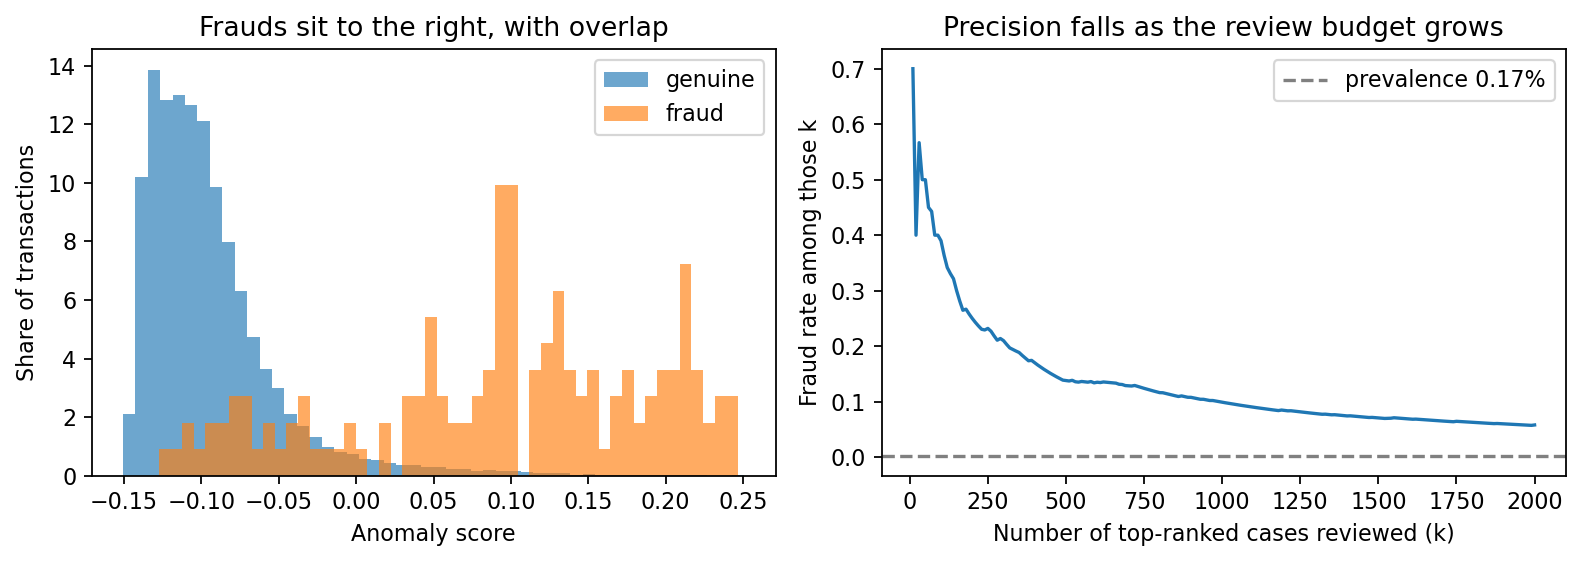
\includegraphics[width=.88\linewidth,height=5cm,keepaspectratio]{labs/visuals/05-notebook-reference.png}
\end{labvisual}

\textbf{What it means.} Fraud scores sit to the right, but non-fraud rows outnumber them about 65 to 1, so even a small overlap produces many false alarms. That is how ROC AUC can look excellent while precision is modest. The right-hand curve starts high and decays towards the base rate; a team with a fixed budget should read its expected hit rate off this curve.
\end{labanswer}

\labpart{Part B --- Self-training and active learning with few labels}

\begin{labquestion}{5}{Split the cancer data three ways}
Now the opposite problem: plenty of rows, but labels are expensive. The breast-cancer data is split three ways. The \emph{pool} is where labels can be bought, the \emph{validation} set judges each policy during development, and the \emph{test} set is sealed until both policies are finished.
\end{labquestion}
\begin{labanswer}
\lstinputlisting[style=utppython,firstline=82,lastline=102]{all_experiments/lab05_anomaly_limited_labels_worked.py}
\begin{refoutput}
\begin{lstlisting}[style=utpterminal]
pool: 319  validation: 107  test: 143
\end{lstlisting}
\end{refoutput}

\textbf{What it means.} The validation and test rows always keep their genuine labels, because the policies are judged against those.
\end{labanswer}

\begin{labquestion}{6}{Self-train from 30\% of the labels}
Self-training hides 70\% of the pool labels (scikit-learn uses $-1$ for ``unknown''), fits on the rest, then lets the model label any unlabeled row it is at least 90\% sure about, and refits. It can help when the confident predictions are right; it can also teach the model its own mistakes.
\end{labquestion}
\begin{labanswer}
\lstinputlisting[style=utppython,firstline=104,lastline=114]{all_experiments/lab05_anomaly_limited_labels_worked.py}
\begin{refoutput}
\begin{lstlisting}[style=utpterminal]
labels kept: 89 of 319
self-training validation accuracy: 0.963
\end{lstlisting}
\end{refoutput}

\textbf{What it means.} That sounds good, but is it good compared with what? Your-turn task~2 asks for the baseline this cell does not compute.
\end{labanswer}

\textbf{Connect it to the chapter.} A score is only useful with a threshold you chose, and a limited label budget is the same kind of decision.
% Reused from chapters/17-anomaly-detection.tex
\begin{labvisual}{Recall the chapter model}
\begin{labgraphic}
\begin{tikzpicture}[font=\scriptsize]
\begin{scope}
\draw[draw=UTPMuted,fill=white] (0,0) rectangle (4.2,2.9);
\foreach \p in {(1.5,1.4),(1.8,1.6),(1.6,1.1),(2.0,1.3),(1.3,1.7),(2.2,1.6),(1.9,0.9),
                (1.4,1.25),(2.1,1.1),(1.7,1.45),(2.3,1.35),(1.55,0.85),(2.05,1.65)}
  \fill[UTPBlue] \p circle (2.4pt);
\draw[UTPTeal,thick,dashed] (1.8,1.32) circle (0.95);
\fill[UTPRed] (3.5,2.4) circle (2.8pt);
\fill[UTPRed] (0.5,0.4) circle (2.8pt);
\node[color=UTPRed,anchor=east] at (4.15,2.72) {anomalies};
\node[color=UTPTeal] at (1.8,-0.35) {the "normal" region};
\node[font=\small\bfseries\color{UTPNavy}] at (2.1,3.25) {Distance / density view};
\end{scope}
\begin{scope}[xshift=5.6cm]
\draw[draw=UTPMuted,fill=white] (0,0) rectangle (4.6,2.9);
\draw[-{Stealth[length=2mm]},UTPMuted] (0.3,0.45) -- (4.35,0.45);
\node[color=UTPMuted,anchor=north,inner sep=1pt] at (2.3,0.40) {anomaly score};
\draw[UTPBlue,very thick] plot[smooth,domain=0.4:4.3,samples=60]
  (\x, {0.45+2.0*exp(-((\x-1.3)^2)/0.28)});
\draw[UTPRed,very thick,dashed] (2.85,0.45) -- (2.85,2.6);
\node[color=UTPRed,anchor=west,align=left] at (2.95,2.2) {threshold\\you choose};
\node[color=UTPGreen] at (1.3,2.68) {normal};
\node[color=UTPRed,anchor=west] at (3.1,0.85) {flagged};
\node[font=\small\bfseries\color{UTPNavy}] at (2.3,3.25) {Score-and-threshold view};
\end{scope}
\end{tikzpicture}
\end{labgraphic}\end{labvisual}


\begin{labquestion}{7}{Simulate active learning}
Active learning chooses \emph{which} labels to buy. Both policies start from the same 40 labels and buy 15 more per round. Uncertainty sampling asks for the rows whose predicted probability is closest to 0.5, where the model is least sure. Random querying is the control: same budget, no strategy.
\end{labquestion}
\begin{labanswer}
\lstinputlisting[style=utppython,firstline=116,lastline=145]{all_experiments/lab05_anomaly_limited_labels_worked.py}
\begin{refoutput}
\begin{lstlisting}[style=utpterminal]
round 1: labels= 40  uncertainty=0.944  random=0.944
round 2: labels= 55  uncertainty=0.925  random=0.953
round 3: labels= 70  uncertainty=0.981  random=0.963
round 4: labels= 85  uncertainty=0.953  random=0.963
round 5: labels=100  uncertainty=0.953  random=0.953
round 6: labels=115  uncertainty=0.953  random=0.953
round 7: labels=130  uncertainty=0.953  random=0.963
round 8: labels=145  uncertainty=0.953  random=0.963
\end{lstlisting}
\end{refoutput}

\textbf{What it means.} No line differs by more than three rows out of 107 (one row is 0.009), so this is mostly noise. Neither policy pulls clearly ahead.
\end{labanswer}

\begin{labquestion}{8}{Plot label efficiency}
Put both curves on one chart, so that the whole run can be read at a glance.
\end{labquestion}
\begin{labanswer}
\lstinputlisting[style=utppython,firstline=147,lastline=156]{all_experiments/lab05_anomaly_limited_labels_worked.py}

\textbf{What it means.} Both curves start at the same point and flatten within a few rounds. This table is simply easy: 40 labels already give a good linear model, so no policy has much left to gain. Active learning earns its keep where the boundary is genuinely uncertain.
\end{labanswer}

\begin{labquestion}{9}{Open the test set once for each policy}
Both policies are finished, so the test set is opened once for each.
\end{labquestion}
\begin{labanswer}
\lstinputlisting[style=utppython,firstline=158,lastline=164]{all_experiments/lab05_anomaly_limited_labels_worked.py}
\begin{refoutput}
\begin{lstlisting}[style=utpterminal]
final test accuracy, uncertainty sampling: 0.972
final test accuracy, random querying:     0.972
\end{lstlisting}
\end{refoutput}

\textbf{What it means.} A tie. Uncertainty sampling did not win, because this dataset is too easy for the policy to matter. The Try-it starts from fewer labels to look for the regime where it does help.
\end{labanswer}

\labpart{Evidence}

\begin{labquestion}{10}{Save the evidence}
Write the numbers above to the results folder. These files are regenerated on every run, so do not edit them by hand.
\end{labquestion}
\begin{labanswer}
\lstinputlisting[style=utppython,firstline=166,lastline=179]{all_experiments/lab05_anomaly_limited_labels_worked.py}
\begin{refoutput}
\begin{lstlisting}[style=utpterminal]
Saved: ['active_learning_curve.csv', 'active_learning_from_20_labels.png',
 'label_efficiency_during_development.png', 'metrics.csv',
 'precision_falls_as_the_review_budget_grows.png', 'top_ranked_transactions.csv']
\end{lstlisting}
\end{refoutput}
\end{labanswer}

\labpart{Try it yourself}

\begin{labquestion}{11}{Try it yourself}
Change the review budget in Part~A to 50 and to 300, and report the fraud rate in each list. Then start the active-learning simulation from 10 labels per class instead of 20, and see whether uncertainty sampling pulls ahead. Attempt it in this empty cell before reading the solution.
\end{labquestion}

\begin{labquestion}{12}{One solution}
Two more review budgets, then the active-learning simulation restarted from 10 labels per class.
\end{labquestion}
\begin{labanswer}
\lstinputlisting[style=utppython,firstline=183,lastline=218]{all_experiments/lab05_anomaly_limited_labels_worked.py}
\noindent\textbf{Continue the same step.}
\lstinputlisting[style=utppython,firstline=219,lastline=221]{all_experiments/lab05_anomaly_limited_labels_worked.py}
\begin{refoutput}
\begin{lstlisting}[style=utpterminal]
top  50 reviewed: fraud rate = 28.0%  (14 frauds found)
top 100 reviewed: fraud rate = 20.0%  (20 frauds found)
top 300 reviewed: fraud rate = 12.3%  (37 frauds found)
labels= 20  uncertainty=0.935  random=0.935
labels= 35  uncertainty=0.944  random=0.935
labels= 50  uncertainty=0.963  random=0.925
labels= 65  uncertainty=0.953  random=0.925
labels= 80  uncertainty=0.953  random=0.953
labels= 95  uncertainty=0.953  random=0.953
labels=110  uncertainty=0.953  random=0.953
labels=125  uncertainty=0.953  random=0.935
\end{lstlisting}
\end{refoutput}

\textbf{What it means.} A team choosing a budget is choosing a point on that curve. Starting from 20 labels, the policies separate for a few rounds, because with so few labels the boundary is genuinely uncertain, and asking about uncertain cases fixes it faster. By about 80 labels the advantage has gone. Remember the scale: 0.963 against 0.925 is four rows of 107.
\end{labanswer}

\begin{yourturn}
Add new cells at the end of the notebook for these tasks, and record your numbers before reading the expected findings.
\begin{enumerate}
  \item \textbf{What would labels buy?} Fit a plain logistic regression on the fraud training rows, this time using the labels. Compare its ROC AUC, average precision and frauds in the top 100 with the Isolation Forest's.
  \item \textbf{Did the unlabeled rows help?} Using the same \texttt{y\_partial} mask as Question~6, fit the plain model on the 89 kept labels only, and score it on the same validation rows. Then fit it on all 319. Compare with self-training's 0.963.
  \item \textbf{Choose a budget.} Suppose reviewing a case costs \$5 and catching a fraud saves \$200. Using the frauds found at budgets of 50, 100, 200, 300, 500 and 1,000 (14, 20, 32, 37, 42 and 45), compute the net saving at each. Which budget would you choose?
\end{enumerate}
\end{yourturn}

\begin{expectedfindings}
\begin{enumerate}
  \item Logistic regression with labels: ROC AUC 0.991, average precision 0.713, 39 of 45 frauds in the top 100. Isolation Forest without labels: 0.952, 0.225, 20 of 45. When labels exist, use them. The anomaly detector's value is for when they do not, or for new kinds of fraud labels cannot describe yet.
  \item Labels only, on 89 rows: 0.972. All 319 labels: 0.972. Self-training: 0.963. The unlabeled rows did not help on this table, and 89 labels were already enough. Always compute this baseline before reporting a semi-supervised method.
  \item Net savings are \$2,550, \$3,500, \$5,400, \$5,900, \$5,900 and \$4,000. Budgets of 300 and 500 tie for best, so the cheaper 300 is the better choice, given these costs. Change the costs, and the answer moves.
\end{enumerate}
\end{expectedfindings}

\begin{troubleshoot}
\begin{description}
  \item[ROC AUC near 0.05 instead of 0.95] You dropped the minus sign in front of \texttt{decision\_function}. Low values mean unusual, so the ranking came out upside down.
  \item[\texttt{SelfTrainingClassifier} rejects your labels] The unlabeled marker must be $-1$, and the labels must be integers. Check \texttt{y\_partial} with \texttt{np.unique}.
  \item[Self-training or active-learning numbers differ on rerun] \texttt{y\_partial} and the first 40 labels draw from the same generator, \texttt{rng}, which keeps moving. Running cells out of order changes both. Restart and run all.
  \item[All frauds appear in the top 100 of your list] You ranked on a column containing the label. The features must not include \texttt{is\_fraud}.
\end{description}
\end{troubleshoot}

\begin{labchecklists}
\begin{verification}
\begin{itemize}
  \item The fraud labels are held back while the Isolation Forest is fitted, and used only to evaluate it.
  \item Precision at the actual review budget is reported alongside ROC AUC, and you can explain why they tell different stories.
  \item Self-training and active learning are judged on the same fixed validation and test sets, with genuine labels.
  \item Uncertainty sampling is compared with random queries at equal label budgets, and small gaps are read against the size of one row.
\end{itemize}
\end{verification}

\begin{labdeliverable}
\begin{itemize}
  \item Restart the kernel and run all cells without errors.
  \item Submit the executed notebook, including your \emph{Your turn} cells, and the generated \texttt{results/lab05/} folder.
  \item Add a short conclusion: the review budget you would recommend and why, and whether the unlabeled rows were worth using on this table.
\end{itemize}
\end{labdeliverable}
\end{labchecklists}

